%\documentclass{jss}
\documentclass[nojss]{jss}
\usepackage[OT1]{fontenc}
\usepackage[latin1]{inputenc}
\usepackage{graphicx}
\usepackage{amsmath}

%\usepackage{cite}
%\usepackage{draftwatermark}
%\SetWatermarkText{Very draft}
%\SetWatermarkScale{1.0}

%\usepackage{myVignette}

\usepackage{ifpdf}
\newcommand*{\Sconcordance}[1]{%
  \ifpdf
    \special{#1}%
  \else
    \immediate\pdfobj{#1}%
  \fi
}

%dimensione figure
\setkeys{Gin}{width=0.8\textwidth}

%\VignetteIndexEntry{An introduction to markovchain package}
%\VignetteKeywords{vig1}
%\VignettePackage{lifecontingencies}
% need no \usepackage{Sweave.sty}

%\SweaveOpts{prefix.string=Figures/fig}
%%%%%%%%%%%%%%%%%%%%%%%%%%%%%%
%% declarations for jss.cls %%%%%%%%%%%%%%%%%%%%%%%%%%%%%%%%%%%%%%%%%%
%%%%%%%%%%%%%%%%%%%%%%%%%%%%%%

%% almost as usual


\author{Giorgio Alfredo Spedicato, Tae Seung Kang, and Sai Bhargav Yalamanchi}

\title{The \pkg{markovchain} Package: A Package for Easily Handling Discrete
Markov Chains in \proglang{R}}

%% for pretty printing and a nice hypersummary also set:
\Plainauthor{Giorgio Alfredo Spedicato, Tae Seung Kang, Sai Bhargav Yalamanchi} %% comma-separated
\Plaintitle{The markovchain Package: A Package for Easily Handling Discrete
Markov Chains in R} %% without formatting
\Shorttitle{The markovchain package} %% a short title (if necessary)
%% an abstract and keywords
\Abstract{The \pkg{markovchain} package aims to fill a gap within
the \proglang{R} framework providing S4 classes and methods for easily handling
discrete time Markov chains, homogeneous and simple inhomogeneous ones.
The S4 classes for handling and analysing discrete time Markov chains are presented, as well as 
functions and method for performing probabilistic and statistical analysis.
Finally, some examples in which the package's functions are applied to Economics, Finance and Natural Sciences topics are shown.}
\Keywords{discrete time Markov chains, transition matrices, communicating classes, periodicity, first passage time, stationary distributions.}
\Plainkeywords{discrete time Markov chains, markovchain, transition matrices, communicating classes, periodicity, first passage time, stationary distributions.} %% without formatting
%% at least one keyword must be supplied



%% publication information
%% NOTE: Typically, this can be left commented and will be filled out by the technical editor
%% \Volume{13}
%% \Issue{9}
%% \Month{September}
%% \Year{2004}
%% \Submitdate{2004-09-29}
%% \Acceptdate{2004-09-29}

%% The address of (at least) one author should be given
%% in the following format:
\Address{
  Giorgio Alfredo Spedicato\\
  Ph.D C.Stat ACAS\\
  UnipolSai R\&D\\
  Via Firenze 11, Paderno Dugnano
  20037 Italy\\
  Telephone: +39/334/6634384\\
  E-mail: \email{spedygiorgio@gmail.com}\\
  URL: \url{www.statisticaladvisor.com}\\
  
  Tae Seung Kang\\
  Ph.D student\\
  Computer \& Information Science \& Engineering\\
  University of Florida\\
  Gainesville, FL, USA\\
  E-mail: \email{tskang3@gmail.com}\\
  
  Sai Bhargav Yalamanchi\\
  B-Tech student\\
  Electrical Engineering\\
  Indian Institute of Technology, Bombay\\
  Mumbai - 400 076, India\\
  E-mail: \email{bhargavcoolboy@gmail.com}\\
}

%% for those who use Sweave please include the following line (with % symbols):
%% need no \usepackage{Sweave.sty}

%% end of declarations %%%%%%%%%%%%%%%%%%%%%%%%%%%%%%%%%%%%%%%%%%%%%%%

\begin{document}
\Sconcordance{concordance:an_introduction_to_markovchain_package.tex:an_introduction_to_markovchain_package.Rnw:%
1 105 1 1 6 197 1 1 2 4 0 1 2 5 1 1 2 11 0 1 1 8 0 1 2 20 1 1 %
2 1 0 1 1 1 4 3 0 1 2 4 0 1 2 2 1 1 6 8 0 1 2 2 1 1 2 4 0 1 2 %
10 1 1 3 5 0 1 2 37 1 1 2 1 0 3 1 6 0 1 1 7 0 1 2 2 1 1 2 1 0 %
3 1 8 0 1 1 9 0 1 2 3 1 1 2 6 0 1 1 5 0 1 1 6 0 1 2 2 1 1 2 6 %
0 1 1 6 0 1 2 8 1 1 2 9 0 1 1 13 0 1 2 2 1 1 3 1 2 6 1 2 2 17 %
1 1 2 1 0 2 1 14 0 1 1 1 2 1 4 3 0 3 1 13 0 1 2 2 1 1 7 6 0 5 %
1 31 0 2 1 13 0 1 2 2 1 1 4 1 2 7 1 1 2 1 0 2 1 13 0 1 2 21 1 %
1 11 43 0 1 2 3 1 1 2 13 0 1 1 6 0 1 2 86 1 1 2 8 0 1 2 10 1 1 %
2 8 0 1 2 2 1 1 15 14 0 1 2 1 1 8 0 1 2 2 1 1 2 6 0 1 1 6 0 1 %
2 3 1 1 35 37 0 1 2 13 1 1 2 1 0 12 1 1 2 1 0 1 1 20 0 1 1 16 %
0 1 2 4 1 1 2 7 0 1 2 2 1 1 2 1 0 1 1 30 0 1 1 31 0 1 2 3 1 1 %
2 6 0 1 1 6 0 1 2 6 1 1 3 1 0 4 1 1 4 2 0 1 1 5 0 1 1 6 0 1 2 %
4 1 1 2 1 0 7 1 1 2 4 0 1 2 2 1 2 2 4 1 1 2 13 0 1 2 4 1 1 11 %
13 0 1 2 2 1 1 3 2 0 1 1 6 0 1 2 31 1 1 2 1 0 1 1 10 0 1 2 3 1 %
1 3 2 0 1 1 16 0 1 2 22 1 1 3 2 0 1 1 12 0 1 1 9 0 1 2 11 1 1 %
4 3 0 1 1 13 0 1 2 6 1 1 2 10 0 1 2 23 1 1 3 2 0 1 1 12 0 1 1 %
9 0 1 2 2 1 1 4 3 0 2 1 3 0 1 2 5 1 1 2 4 0 1 2 11 1 1 2 6 0 1 %
1 6 0 1 2 10 1 1 2 19 0 1 1 19 0 1 2 4 1 1 4 22 0 1 2 6 1 1 2 %
1 0 3 1 13 0 1 2 18 1 1 3 8 0 1 2 5 1 1 2 7 0 1 2 6 1 1 2 7 0 %
1 2 18 1 1 6 7 0 1 2 3 1 1 2 1 0 1 1 6 0 1 2 6 0 1 2 7 0 1 2 2 %
1 1 2 1 0 1 1 7 0 1 2 2 1 1 2 1 0 1 1 7 0 1 2 3 1 1 2 1 0 1 1 %
6 0 1 2 1 1 7 0 1 2 7 1 1 2 1 0 1 1 7 0 1 2 2 1 1 2 1 0 1 1 13 %
0 1 2 2 1 1 2 8 0 1 2 11 1 1 3 1 0 1 9 11 0 1 2 2 1 1 3 2 0 1 %
1 6 0 1 2 26 1 1 2 1 0 4 1 3 0 1 2 2 1 1 2 1 0 1 1 3 0 1 2 2 1 %
1 2 7 0 1 2 25 1 1 26 28 0 1 3 2 1 1 2 1 0 1 1 6 0 1 2 3 1 1 2 %
7 0 1 2 10 1 1 8 6 0 1 1 3 0 1 2 2 1 1 2 1 0 3 1 3 0 1 2 2 1 1 %
4 6 0 1 2 2 1 1 2 4 0 1 2 2 1 1 2 1 0 3 1 7 0 1 2 4 1 1 2 1 0 %
2 1 14 0 1 2 4 1 1 3 1 2 7 1 1 2 8 0 1 2 13 1 1 2 4 0 1 2 2 1 %
1 3 2 0 1 1 14 0 1 2 6 1 1 4 3 0 7 1 13 0 1 2 3 1 1 2 1 0 1 1 %
3 0 2 2 1 0 1 1 8 0 3 1 3 0 1 2 27 1}



\maketitle

\section{Introduction}
Markov chains represent a class of stochastic processes of great interest for the wide spectrum of practical applications.
In particular, discrete time Markov chains (DTMC) permit to model the transition probabilities between discrete states by the aid of matrices.
Various \proglang{R} packages deal with models that are based on Markov chains:
\begin{itemize}
\item \pkg{msm} \citep{msmR} handles Multi-State Models for panel data;
\item \pkg{mcmcR} \citep{mcmcR} implements Monte Carlo Markov Chain approach;  \item \pkg{hmm} \citep{hmmR} fits hidden Markov models with covariates;
\item \pkg{mstate} fits 
Multi-State Models based on Markov chains for survival analysis \citep{mstateR}.
\end{itemize}
Nevertheless, the \proglang{R} statistical environment \citep{rSoftware} seems to lack a simple package that coherently defines S4 classes for discrete Markov chains and allows to perform probabilistic analysis, statistical inference and
applications. For the sake of completeness, \pkg{markovchain} is the second package specifically dedicated to DTMC analysis, being \pkg{DTMCPack} \citep{DTMCPackR} the first one. Notwithstanding, \pkg{markovchain} package \citep{markovchainR} aims to offer
more flexibility in handling DTMC than other existing
solutions, providing S4 classes for both homogeneous and non-homogeneous Markov chains as well as methods suited to perform statistical and probabilistic analysis.\\
The \pkg{markovchain} package depends on the following \proglang{R} packages: \pkg{expm} \citep{expmR} to perform efficient matrices powers; \pkg{igraph} \citep{pkg:igraph} to perform pretty plotting of \code{markovchain} objects and \pkg{matlab} \citep{pkg:matlab}, that contains functions for matrix management and calculations that emulate those within \proglang{MATLAB} environment.
Moreover, other scientific softwares provide functions specifically designed
to analyze DTMC, as \proglang{Mathematica} 9 \citep{mathematica9}.\\
The paper is structured as follows: 
Section~\ref{sec:mathematic} briefly reviews mathematics and 
definitions regarding DTMC, Section~\ref{sec:structure}
discusses how to handle and manage Markov chain objects within the package,
Section~\ref{sec:probability} and Section~\ref{sec:statistics} show how to
perform probabilistic and statistical modelling, while
Section~\ref{sec:applications} presents some applied examples from various
fields analyzed by means of the \pkg{markovchain} package.

\section{Review of core mathematical concepts}\label{sec:mathematic}

\subsection{General Definitions}

A DTMC is a sequence of random variables $X_{1},\: X_{2}\: ,\ldots,\:X_{n},\ldots$ characterized by the Markov property (also known as memoryless property, see
Equation~\ref{eq:markovProp}). The Markov property states that the distribution of the forthcoming state $X_{n+1}$ depends only on the current state $X_{n}$ and doesn't depend on the previous ones $X_{n-1},\: X_{n-2},\ldots,\: X_{1}$.

\begin{equation}
Pr\left(X_{n+1}=x_{n+1}\left|X_{1}=x_{1},X_{2}=x_{2,}...,X_{n}=x_{n}\right.\right)=Pr\left(X_{n+1}=x_{n+1}\left|X_{n}=x_{n}\right.\right).
\label{eq:markovProp}
\end{equation}

The set of possible states $S=\left\{ s_{1},s_{2},...,s_{r}\right\}$ of $X_{n}$ can be finite or countable and it is named the state space of the chain.

The chain moves  from one state to another (this change
is named either 'transition' or 'step') and the probability $p_{ij}$ to move
from state $s_{i}$ to state $s_{j}$ in one step is named transition probability:

\begin{equation}
p_{ij}=Pr\left(X_{1}=s_{j}\left|X_{0}=s_{i}\right.\right).
\label{eq:trProp}
\end{equation}

The probability of moving from state $i$ to $j$ in $n$ steps is denoted by
$p_{ij}^{(n)}=Pr\left(X_{n}=s_{j}\left|X_{0}=s_{i}\right.\right)$. 

A DTMC is called time-homogeneous if the property shown in Equation~\ref{eq:mcHom} holds. Time homogeneity implies no change in the underlying transition probabilities as time goes on.
\begin{equation}
Pr\left(X_{n+1}=s_{j}\left|X_{n}=s_{i}\right.\right)=Pr\left(X_{n}=s_{j}\left|X_{n-1}=s_{i}\right.\right).
\label{eq:mcHom}
\end{equation}

If the Markov chain is time-homogeneous, then $p_{ij}=Pr\left(X_{k+1}=s_{j}\left|X_{k}=s_{i}\right.\right)$
and \\ $p_{ij}^{(n)}=Pr\left(X_{n+k}=s_{j}\left|X_{k}=s_{i}\right.\right)$,
where $k>0$.

The probability distribution of transitions from one state to another
can be represented into a transition matrix $P=(p_{ij})_{i,j}$, where each element
of position $(i,j)$ represents the transition probability $p_{ij}$. E.g., if
$r=3$ the transition matrix $P$ is shown in Equation~\ref{eq:trPropEx}

\begin{equation}
P=\left[\begin{array}{ccc}
p_{11} & p_{12} & p_{13}\\
p_{21} & p_{22} & p_{23}\\
p_{31} & p_{32} & p_{33}
\end{array}\right].
\label{eq:trPropEx}
\end{equation}


The distribution over the states can be written in the form of a stochastic row
vector $x$ (the term stochastic means that $\sum_{i}x_{i}=1, x_{i} \geq 0$): e.g., if the current state of $x$ is $s_{2}$, $x=\left(0\:1\:0\right)$.
As a consequence, the relation between $x^{(1)}$ and $x^{(0)}$
is $x^{(1)}=x^{(0)}P$ and, recursively, we get $x^{(2)}=x^{(0)}P^{2}$ and
$x^{(n)}=x^{(0)}P^{n},\, n>0$.

DTMC are explained in most theory books on stochastic processes, see \cite{bremaud1999discrete} and \cite{ching2006markov} for example. Valuable references online available are: \cite{konstantopoulos2009markov}, \cite{probBook} and \cite{bardPpt}.


\subsection{Properties and classification of states}\label{sec:properties}

A state $s_{j}$ is said accessible from state $s_{i}$ (written $s_{i}\rightarrow s_{j}$) if a system started in state $s_{i}$ has
a positive probability to reach the state $s_{j}$ at a certain
point, i.e., $\exists n>0:\: p_{ij}^{n}>0$. If both $s_{i}\rightarrow s_{j}$ and $s_{j}\rightarrow s_{i}$, then
$s_{i}$ and $s_{j}$ are said to communicate.

A communicating class is defined to be a set of states that communicate. 
A DTMC can be composed by one or more communicating classes.  If the DTMC is
composed by only one communicating class (i.e., if all states in the chain communicate), then
it is said irreducible. A communicating class is said to be closed if no states outside of the class can be reached from any state inside it.

If $p_{ii}=1$, $s_{i}$ is defined as absorbing
state: an absorbing state corresponds to a closed communicating class composed by one state only.

The canonic form of a DTMC transition matrix is a matrix having a
block form, where the closed communicating classes are shown at the beginning of the diagonal matrix.

A state $s_{i}$ has period $k_{i}$ if any return to state $s_{i}$
must occur in multiplies of $k_{i}$ steps, that is $k_{i}=gcd\left\{ n:Pr\left(X_{n}=s_{i}\left|X_{0}=s_{i}\right.\right)>0\right\}$, where
$gcd$ is the greatest common divisor. If $k_{i}=1$ the state $s_{i}$ is said
to be aperiodic, else if $k_{i}>1$ the state $s_{i}$ is periodic with period $k_{i}$. Loosely speaking, $s_{i}$  is periodic if it can only return to itself after a fixed number of transitions $k_{i}>1$ (or multiple of $k_{i}$), else it is aperiodic. 

If states $s_{i}$ and $s_{j}$ belong to the same communicating class, then they have the same period $k_{i}$. As a consequence, each of the states of an irreducible DTMC share the same periodicity. This periodicity is also considered the DTMC periodicity.

It is possible to analyze the timing to reach a certain state. The first passage time from state $s_{i}$ to state $s_{j}$ is the number $T_{ij}$ of steps taken by the chain until it arrives for the first time to state $s_{j}$, given that $X_{0} = s_{i}$. The probability distribution of $T_{ij}$ is defined by Equation~\ref{eq:fpt1}

\begin{equation}
{h_{ij}}^{\left( n \right)} = Pr\left( {{T_{ij}} = n} \right) = Pr\left( {{X_n} = s_{j},{X_{n - 1}} \ne s_{j}, \ldots ,{X_1} \ne s_{j}|{X_0} = s_{i}} \right)
\label{eq:fpt1}
\end{equation}

and can be found recursively using Equation~\ref{eq:ftp2}, given that ${h_{ij}}^{\left( n \right)} = p_{ij}$.

\begin{equation}
{h_{ij}}^{\left( n \right)} = \sum\limits_{k \in S - \left\{ s_{j} \right\}}^{} {{p_{ik}}{h_{kj}}^{\left( {n - 1} \right)}}.
\label{eq:ftp2}
\end{equation}

If in the definition of the first passage time we let $s_{i}=s_{j}$, we obtain the first return time $T_{i}=inf \{ n\geq1:X_{n}=s_{i}|X_{0}=s_{i} \}$. A state $s_{i}$ is said to be recurrent if it is visited infinitely often, i.e., $Pr(T_{i}<+\infty|X_{0}=s_{i})=1$. On the opposite, $s_{i}$ is called transient if there is a positive probability that the chain will never return to $s_{i}$, i.e., $Pr(T_{i}=+\infty|X_{0}=s_{i})>0$. 

Given a time homogeneous Markov chain with transition matrix \emph{P},
a stationary distribution \emph{z} is a stochastic row vector such that $z=z\cdot P$, where $0\leq z_{j}\leq 1 \: \forall j$ and
$\sum_{j}z_{j}=1$.

If a DTMC $\{X_{n}\}$ is irreducible and aperiodic, then it has a limit distribution and this distribution is stationary. As a consequence, if $P$
is the $k\times k$ transition matrix of the chain and $z=\left(z_{1},...,z_{k}\right)$ is the eigenvector of $P$ such that $\sum_{i=1}^{k}z_{i}=1$, then we get

\begin{equation}
  \underset{n\rightarrow\infty}{lim}P^{n}=Z,
  \label{eq:limMc}
\end{equation}


where $Z$ is the matrix having all rows equal to $z$. The stationary distribution of $\{X_{n}\}$ is represented by $z$.


\subsection{A short example}

Consider the following numerical example. Suppose we have a DTMC with a set of 3 possible states $S=\{s_{1}, s_{2}, s_{3}\}$.
Let the transition matrix be 
\begin{equation}
P=\left[\begin{array}{ccc}
0.5 & 0.2 & 0.3\\
0.15 & 0.45 & 0.4\\
0.25 & 0.35 & 0.4
\end{array}\right].
\label{eq:trPropExEx1}
\end{equation}

In $P$, $p_{11}=0.5$ is the probability that $X_{1}=s_{1}$ given
that we observed $X_{0}=s_{1}$ is 0.5, and so on. 
It is easy to see that the chain is irreducible since all the states communicate (it is made by one communicating class only).

Suppose that the current state of the chain is $X_{0}=s_{2}$, i.e., $x^{(0)}=(0\:1\:0)$, then the probability distribution of states after 1 and 2 steps can be computed as shown in Equations~\ref{eq:trPropExEx2} and
~\ref{eq:trPropExEx3}.

\begin{equation}
x^{(1)}=\left(0\:1\:0\right)\left[\begin{array}{ccc}
0.5 & 0.2 & 0.3\\
0.15 & 0.45 & 0.4\\
0.25 & 0.35 & 0.4
\end{array}\right]=\left(0.15\:0.45\:0.4\right).
\label{eq:trPropExEx2}
\end{equation}


\begin{equation}
x^{(n)}=x^{(n-1)}P \to \left(0.15\:0.45\:0.4\right)\left[\begin{array}{ccc}
0.5 & 0.2 & 0.3\\
0.15 & 0.45 & 0.4\\
0.25 & 0.35 & 0.4
\end{array}\right]=\left(0.2425\:0.3725\:0.385\right).
\label{eq:trPropExEx3}
\end{equation}


If, f.e., we are interested in the probability of reaching the state $s_{3}$ in two steps, then $Pr\left(X_{2}=s_{3}\left|X_{0}=s_{2}\right.\right)=0.385$.

\newpage

\section{The structure of the package}\label{sec:structure}



\subsection{Creating markovchain objects}

The package is loaded within the \proglang{R} command line as follows:

\begin{Schunk}
\begin{Sinput}
R> library("markovchain")
\end{Sinput}
\end{Schunk}



The \code{markovchain} and  \code{markovchainList}  S4 classes \citep{chambers}
are defined within the \pkg{markovchain} package as displayed:

\begin{Schunk}
\begin{Soutput}
Class "markovchain" [package "markovchain"]

Slots:
                                                         
Name:            states            byrow transitionMatrix
Class:        character          logical           matrix
                       
Name:              name
Class:        character
\end{Soutput}
\begin{Soutput}
Class "markovchainList" [package "markovchain"]

Slots:
                                
Name:  markovchains         name
Class:         list    character
\end{Soutput}
\end{Schunk}

The first class has been designed to handle homogeneous Markov chain processes,
while the latter (which is itself a list of \code{markovchain} objects) has been
designed to handle non-homogeneous Markov chains processes.

Any element of \code{markovchain} class is comprised by following slots:
\begin{enumerate}
  \item \code{states}: a character vector, listing the states for which transition probabilities are defined.
  \item \code{byrow}: a logical element, indicating whether transition probabilities are shown by row or by column.
  \item \code{transitionMatrix}: the probabilities of the transition matrix.
  \item \code{name}: optional character element to name the DTMC.
\end{enumerate}

The \code{markovchainList} objects are defined by following slots:
\begin{enumerate}
  \item \code{markovchains}: a list of \code{markovchain} objects.
  \item \code{name}: optional character element to name the DTMC.
\end{enumerate}

The \code{markovchain} objects can be created either in a long way, as the following code shows

\begin{Schunk}
\begin{Sinput}
R> weatherStates <- c("sunny", "cloudy", "rain")
R> byRow <- TRUE
R> weatherMatrix <- matrix(data = c(0.70, 0.2, 0.1,
+                         0.3, 0.4, 0.3,
+                         0.2, 0.45, 0.35), byrow = byRow, nrow = 3,
+                       dimnames = list(weatherStates, weatherStates))
R> mcWeather <- new("markovchain", states = weatherStates, byrow = byRow, 
+                 transitionMatrix = weatherMatrix, name = "Weather")
\end{Sinput}
\end{Schunk}

or in a shorter way, displayed below

\begin{Schunk}
\begin{Sinput}
R> mcWeather <- new("markovchain", states = c("sunny", "cloudy", "rain"),
+                   transitionMatrix = matrix(data = c(0.70, 0.2, 0.1,
+                         0.3, 0.4, 0.3,
+                         0.2, 0.45, 0.35), byrow = byRow, nrow = 3), 
+                   name = "Weather")
\end{Sinput}
\end{Schunk}

When \code{new("markovchain")} is called alone, a default Markov chain is created.

\begin{Schunk}
\begin{Sinput}
R> defaultMc <- new("markovchain")
\end{Sinput}
\end{Schunk}

The quicker way to create \code{markovchain} objects is made possible thanks to
the implemented \code{initialize} S4 method that checks that:

\begin{itemize}
  \item the \code{transitionMatrix} to be a transition matrix, i.e., all entries to be probabilities and either all rows or all columns to sum up to one.
  \item the columns and rows names of \code{transitionMatrix} to be defined and to coincide with \code{states} vector slot. 
\end{itemize}

The \code{markovchain} objects can be collected in a list within \code{markovchainList} S4 objects as following example shows.

\begin{Schunk}
\begin{Sinput}
R> mcList <- new("markovchainList", markovchains = list(mcWeather, defaultMc), 
+  		name = "A list of Markov chains")
\end{Sinput}
\end{Schunk}



\subsection{Handling markovchain objects}

Table~\ref{tab:methodsToHandleMc} lists which methods handle and 
manipulate \code{markovchain} objects.

\begin{table}[h]
  \centering
  \begin{tabular}{lll}
    \hline
  Method & Purpose \\
    \hline  \hline
  \code{*} & Direct multiplication for transition matrices.\\
%  $\^$ & Integer power of a markov chain.\\
  \code{[} & Direct access to the elements of the transition matrix.\\
  \code{==} & Equality operator between two transition matrices.\\
  \code{as} & Operator to convert \code{markovchain} objects into \code{data.frame} and\\
  & \code{table} object.\\
\code{dim} & Dimension of the transition matrix.\\
\code{plot} & \code{plot} method for \code{markovchain} objects.\\
\code{print} & \code{print} method for \code{markovchain} objects.\\
\code{show} & \code{show} method for \code{markovchain} objects.\\
  \code{states} & Name of the transition states.\\
  \code{t} & Transposition operator (which switches byrow slot value and modifies \\
 &  the transition matrix coherently).\\
  \hline
\end{tabular}
\caption{\pkg{markovchain} methods for handling \code{markovchain} objects.}
\label{tab:methodsToHandleMc}
\end{table}  


The examples that follow shows how operations on \code{markovchain} objects can be easily performed. 
For example, using the previously defined matrix we can find what is the probability distribution of expected weather states in two and  seven days, given the actual state to be cloudy. 

\begin{Schunk}
\begin{Sinput}
R> initialState <- c(0, 1, 0)
R> after2Days <- initialState * (mcWeather * mcWeather)
R> after7Days <- initialState * (mcWeather ^ 7)
R> after2Days
\end{Sinput}
\begin{Soutput}
     sunny cloudy  rain
[1,]  0.39  0.355 0.255
\end{Soutput}
\begin{Sinput}
R> round(after7Days, 3)
\end{Sinput}
\begin{Soutput}
     sunny cloudy  rain
[1,] 0.462  0.319 0.219
\end{Soutput}
\end{Schunk}

A similar answer could have been obtained defining the vector of probabilities as a column vector. A column - defined probability matrix could be set up either creating a new matrix or transposing an existing \code{markovchain} object thanks to the \code{t} method.

\begin{Schunk}
\begin{Sinput}
R> initialState <- c(0, 1, 0)
R> after2Days <- (t(mcWeather) * t(mcWeather)) * initialState
R> after7Days <- (t(mcWeather) ^ 7) * initialState
R> after2Days
\end{Sinput}
\begin{Soutput}
        [,1]
sunny  0.390
cloudy 0.355
rain   0.255
\end{Soutput}
\begin{Sinput}
R> round(after7Days, 3)
\end{Sinput}
\begin{Soutput}
        [,1]
sunny  0.462
cloudy 0.319
rain   0.219
\end{Soutput}
\end{Schunk}

Basic methods have been defined for \code{markovchain} objects to
quickly get states and transition matrix dimension.

\begin{Schunk}
\begin{Sinput}
R> states(mcWeather)
\end{Sinput}
\begin{Soutput}
[1] "sunny"  "cloudy" "rain"  
\end{Soutput}
\begin{Sinput}
R> dim(mcWeather)
\end{Sinput}
\begin{Soutput}
[1] 3
\end{Soutput}
\end{Schunk}

A direct access to transition probabilities is provided both by \code{transitionProbability} method and "[" method.

\begin{Schunk}
\begin{Sinput}
R> transitionProbability(mcWeather, "cloudy", "rain")
\end{Sinput}
\begin{Soutput}
[1] 0.3
\end{Soutput}
\begin{Sinput}
R> mcWeather[2,3]
\end{Sinput}
\begin{Soutput}
[1] 0.3
\end{Soutput}
\end{Schunk}

The transition matrix of a \code{markovchain} object can be displayed using \code{print} or \code{show} 
methods (the latter being less laconic). Similarly, the underlying transition probability diagram 
can be plotted by the use of \code{plot} method (as shown in Figure~\ref{fig:mcPlot}) which is based on \pkg{igraph} package \citep{pkg:igraph}.
\code{plot} method for \code{markovchain} objects is a wrapper of
\code{plot.igraph} for \code{igraph} S4 objects defined within the \pkg{igraph} package. 
Additional parameters can be passed to \code{plot} function to control the network graph layout.

\begin{Schunk}
\begin{Sinput}
R> print(mcWeather)
\end{Sinput}
\begin{Soutput}
       sunny cloudy rain
sunny    0.7   0.20 0.10
cloudy   0.3   0.40 0.30
rain     0.2   0.45 0.35
\end{Soutput}
\begin{Sinput}
R> show(mcWeather)
\end{Sinput}
\begin{Soutput}
Weather 
 A  3 - dimensional discrete Markov Chain with following states 
 sunny cloudy rain 
 The transition matrix   (by rows)  is defined as follows 
       sunny cloudy rain
sunny    0.7   0.20 0.10
cloudy   0.3   0.40 0.30
rain     0.2   0.45 0.35
\end{Soutput}
\end{Schunk}

\begin{figure}
\begin{center}
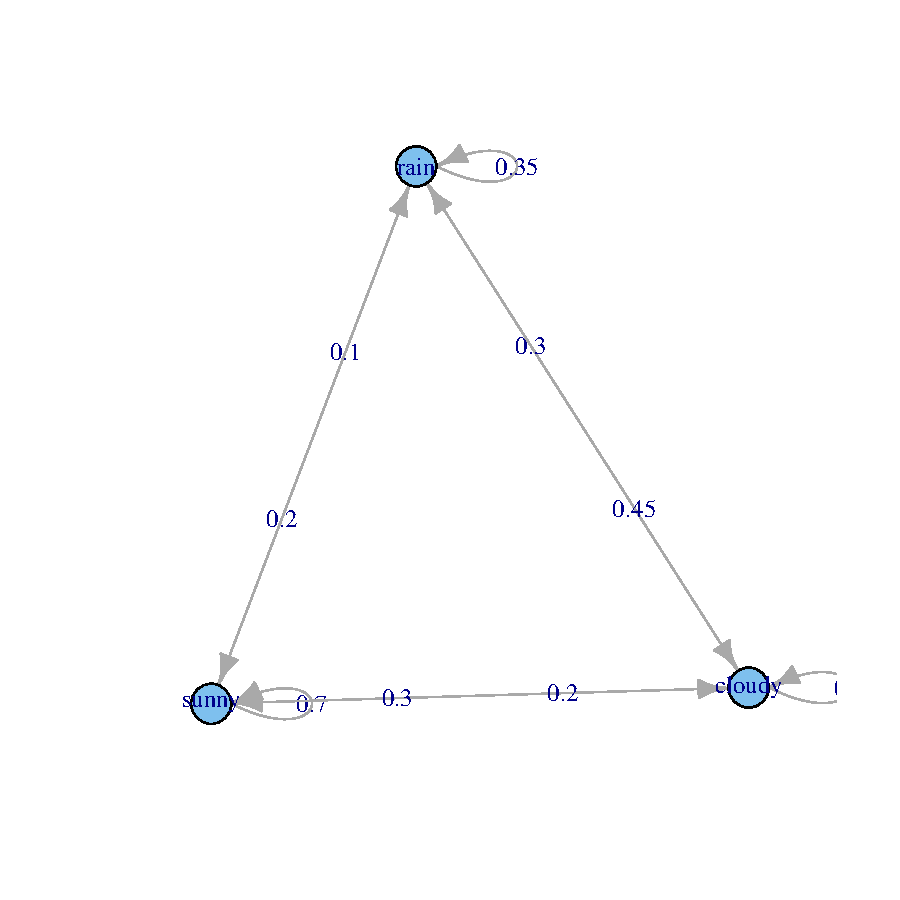
\includegraphics{an_introduction_to_markovchain_package-mcPlot}
\caption{Weather example. Markov chain plot.}
\label{fig:mcPlot}
\end{center}
\end{figure}

Import and export from some specific classes is possible, as shown in
Figure~\ref{fig:fromAndTo} and in the following code.\\

\begin{Schunk}
\begin{Sinput}
R> mcDf <- as(mcWeather, "data.frame")
R> mcNew <- as(mcDf, "markovchain")
R> mcDf
\end{Sinput}
\begin{Soutput}
      t0     t1 prob
1  sunny  sunny 0.70
2  sunny cloudy 0.20
3  sunny   rain 0.10
4 cloudy  sunny 0.30
5 cloudy cloudy 0.40
6 cloudy   rain 0.30
7   rain  sunny 0.20
8   rain cloudy 0.45
9   rain   rain 0.35
\end{Soutput}
\begin{Sinput}
R> mcIgraph <- as(mcWeather, "igraph")
\end{Sinput}
\end{Schunk}

\begin{figure}
\begin{center}
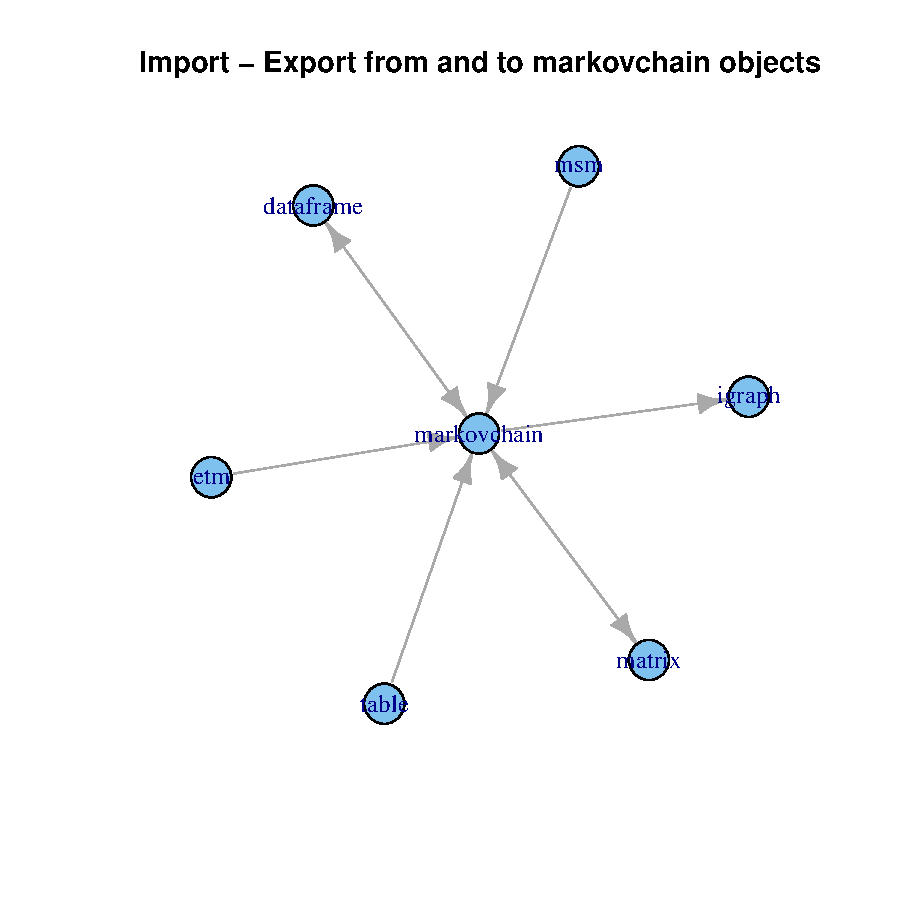
\includegraphics{an_introduction_to_markovchain_package-importExportPlot}
\caption{The \pkg{markovchain} methods for import and export.}
\label{fig:fromAndTo}
\end{center}
\end{figure}


Coerce from \code{matrix} method, as the code below shows, represents another approach to create a \code{markovchain} method starting from a given squared probability matrix.

\begin{Schunk}
\begin{Sinput}
R> myMatr<-matrix(c(.1,.8,.1,.2,.6,.2,.3,.4,.3), byrow=TRUE, ncol=3)
R> myMc<-as(myMatr, "markovchain")
R> myMc
\end{Sinput}
\begin{Soutput}
Unnamed Markov chain 
 A  3 - dimensional discrete Markov Chain with following states 
 s1 s2 s3 
 The transition matrix   (by rows)  is defined as follows 
    s1  s2  s3
s1 0.1 0.8 0.1
s2 0.2 0.6 0.2
s3 0.3 0.4 0.3
\end{Soutput}
\end{Schunk}

% \begin{table}[h]
%   \centering
%   \begin{tabular}{lll}
%     \hline
%   Object & Direction \\
%     \hline  \hline
%   \code{data.frame} & bidirectional \\
%   \code{igraph} & only to igraph\\
%   \code{matrix} & bidirectional\\
%   \code{table} & only from table\\
%   \hline
% \end{tabular}
% \caption{The \pkg{markovchain} methods for import and export.}
% \label{tab:fromAndTo}
% \end{table}  

Non-homogeneous Markov chains can be created with the aid of \code{markovchainList} object. The example that follows arises from health insurance, where the costs associated to patients in a Continuous Care Health Community (CCHC) are modelled by a non-homogeneous Markov Chain, since the 
transition probabilities change by year. Methods explicitly written for
\code{markovchainList} objects are: \code{print}, \code{show},  \code{dim} and
\code{[}.

\begin{Schunk}
\begin{Soutput}
Continuous Care Health Community  list of Markov chain(s) 
Markovchain  1 
state t0 
 A  3 - dimensional discrete Markov Chain with following states 
 H I D 
 The transition matrix   (by rows)  is defined as follows 
    H   I   D
H 0.7 0.2 0.1
I 0.1 0.6 0.3
D 0.0 0.0 1.0

Markovchain  2 
state t1 
 A  3 - dimensional discrete Markov Chain with following states 
 H I D 
 The transition matrix   (by rows)  is defined as follows 
    H   I   D
H 0.5 0.3 0.2
I 0.0 0.4 0.6
D 0.0 0.0 1.0

Markovchain  3 
state t2 
 A  3 - dimensional discrete Markov Chain with following states 
 H I D 
 The transition matrix   (by rows)  is defined as follows 
    H   I   D
H 0.3 0.2 0.5
I 0.0 0.2 0.8
D 0.0 0.0 1.0

Markovchain  4 
state t3 
 A  3 - dimensional discrete Markov Chain with following states 
 H I D 
 The transition matrix   (by rows)  is defined as follows 
  H I D
H 0 0 1
I 0 0 1
D 0 0 1
\end{Soutput}
\end{Schunk}

It is possible to perform direct access to \code{markovchainList} elements, as well as to 
determine the number of \code{markovchain} objects by which a \code{markovchainList} object is composed.

\begin{Schunk}
\begin{Sinput}
R> mcCCRC[[1]]
\end{Sinput}
\begin{Soutput}
state t0 
 A  3 - dimensional discrete Markov Chain with following states 
 H I D 
 The transition matrix   (by rows)  is defined as follows 
    H   I   D
H 0.7 0.2 0.1
I 0.1 0.6 0.3
D 0.0 0.0 1.0
\end{Soutput}
\begin{Sinput}
R> dim(mcCCRC)
\end{Sinput}
\begin{Soutput}
[1] 4
\end{Soutput}
\end{Schunk}

The \code{markovchain} package contains some data found in the
literature related to DTMC models (see Section~\ref{sec:applications}).
Table~\ref{tab:datasets} lists datasets and tables included within the current release of
the package.

\begin{table}[h]
  \centering
  \begin{tabular}{lll}
  \hline
  Dataset & Description \\
 \hline  \hline
  \code{blanden} & Mobility across income quartiles, \cite{blandenEtAlii}.\\
  \code{craigsendi} & CD4 cells, \cite{craigSendi}.\\
  \code{preproglucacon} & Preproglucacon DNA basis, \cite{averyHenderson}.\\
  \code{rain} & Alofi Island rains, \cite{averyHenderson}.\\
  \code{holson} & Individual states trajectiories.\\ 
\hline
\end{tabular}
\caption{The \pkg{markovchain} \code{data.frame} and \code{table}.}
\label{tab:datasets}
\end{table}

Finally, Table~\ref{tab:demos} lists the demos included in the demo directory of the package.

\begin{table}[h]
  \centering
  \begin{tabular}{lll}
    \hline
  Dataset & Description \\
    \hline  \hline
    \code{bard.R} & Structural analysis of Markov chains from Bard PPT.\\
    \code{examples.R} & Notable Markov chains, e.g., The Gambler Ruin chain.\\
    \code{quickStart.R} & Generic examples.\\
\hline
\end{tabular}
\caption{The \pkg{markovchain} demos.}
\label{tab:demos}
\end{table}

\clearpage

\section{Probability with markovchain objects}\label{sec:probability}


The \pkg{markovchain} package contains functions to analyse DTMC from a
probabilistic perspective. For example, the package provides methods to find
stationary distributions and identifying absorbing and transient states. Many of
these methods come from \proglang{MATLAB} listings
that have been ported into \proglang{R}. For a full description of the underlying
theory and algorithm the interested reader can overview the original
\proglang{MATLAB} listings, \cite{renaldoMatlab} and \cite{montgomery}.

Table~\ref{tab:methodsToStats} shows methods that can be applied on \code{markovchain} objects to perform probabilistic analysis. 

\begin{table}[h]
  \centering
  \begin{tabular}{lll}
    \hline
  Method & Returns \\
    \hline  \hline
  \code{absorbingStates} & the absorbing states of the transition
  matrix, if any.\\
\code{conditionalDistribution} & the conditional distribution of the
subsequent state \\
 & $s_{j}$, given actual state $s_{i}$.\\
\code{canonicForm} & the transition matrix into canonic form.\\
\code{is.accessible} & verification if a state j is reachable from state i.\\
\code{is.irreducible} & verification whether a DTMC is irreducible.\\
\code{period} & the period of an irreducible DTMC.\\
\code{steadyStates} & the vector(s) of steady state(s) in matrix
form.\\
\code{summary} & DTMC summary.\\
\code{transientStates} & the transient states of the transition
  matrix, if any.\\
\hline
\end{tabular}
\caption{\pkg{markovchain} methods: statistical operations.}
\label{tab:methodsToStats}
\end{table}


The conditional distribution of weather states, given that current day's weather
is sunny, is given by following code.

\begin{Schunk}
\begin{Sinput}
R> conditionalDistribution(mcWeather, "sunny")
\end{Sinput}
\begin{Soutput}
 sunny cloudy   rain 
   0.7    0.2    0.1 
\end{Soutput}
\end{Schunk}

The steady state(s), also known as stationary distribution(s),  of the Markov
chains are identified by the such described algorithm:
\begin{enumerate}
  \item decompose the transition matrix in eigenvalues and eigenvectors;
  \item consider only eigenvectors corresponding to eigenvalues equal to one;
  \item normalize such eigenvalues so that the sum of their components is one.
\end{enumerate}

The result is returned in matrix form.

\begin{Schunk}
\begin{Sinput}
R> steadyStates(mcWeather)
\end{Sinput}
\begin{Soutput}
         sunny    cloudy      rain
[1,] 0.4636364 0.3181818 0.2181818
\end{Soutput}
\end{Schunk}

It is possible for a Markov chain to have more than one stationary distribution, as the gambler ruin example shows.

\begin{Schunk}
\begin{Sinput}
R> gamblerRuinMarkovChain <- function(moneyMax, prob = 0.5) {
+    require(matlab)
+    matr <- zeros(moneyMax + 1)
+    states <- as.character(seq(from = 0, to = moneyMax, by = 1))
+    rownames(matr) = states; colnames(matr) = states
+    matr[1,1] = 1; matr[moneyMax + 1,moneyMax + 1] = 1
+    for(i in 2:moneyMax)
+    { matr[i,i-1] = 1 - prob; matr[i, i + 1] = prob   }
+    out <- new("markovchain",  
+             transitionMatrix = matr, 
+             name = paste("Gambler ruin", moneyMax, "dim", sep = " ")
+             )
+    return(out)
+  }
R> mcGR4 <- gamblerRuinMarkovChain(moneyMax = 4, prob = 0.5)
R> steadyStates(mcGR4)
\end{Sinput}
\begin{Soutput}
     0 1 2 3 4
[1,] 1 0 0 0 0
[2,] 0 0 0 0 1
\end{Soutput}
\end{Schunk}

Absorbing states are determined by means of \code{absorbingStates} method.

\begin{Schunk}
\begin{Sinput}
R> absorbingStates(mcGR4)
\end{Sinput}
\begin{Soutput}
[1] "0" "4"
\end{Soutput}
\begin{Sinput}
R> absorbingStates(mcWeather)
\end{Sinput}
\begin{Soutput}
character(0)
\end{Soutput}
\end{Schunk}

The key function used within \cite{renaldoMatlab} (and \pkg{markovchain}'s
derived functions) is \\ \code{.commclassKernel}, that is called below.

\begin{Schunk}
\begin{Sinput}
R> .commclassesKernel <- function(P){
+    m <- ncol(P)
+  	stateNames <- rownames(P)
+  	T <- zeros(m) 
+  	i <- 1
+  	while (i <= m) { 
+  		a <- i 
+  		b <- zeros(1,m)
+  		b[1,i] <- 1
+  		old <- 1
+  		new <- 0
+  		while (old != new) {
+  			old <- sum(find(b > 0))
+  			n <- size(a)[2]
+  			matr <- matrix(as.numeric(P[a,]), ncol = m, 
+                       nrow = n)
+  			c <- colSums(matr)
+  			d <- find(c)
+  			n <- size(d)[2]
+  			b[1,d] <- ones(1,n)
+  			new <- sum(find(b>0))
+  			a <- d
+  		}
+  		T[i,] <- b
+  		i <- i+1 }
+  	F <- t(T)  
+  	C <- (T > 0)&(F > 0)
+  	v <- (apply(t(C) == t(T), 2, sum) == m)
+  	colnames(C) <- stateNames
+  	rownames(C) <- stateNames
+  	names(v) <- stateNames
+  	out <- list(C = C, v = v)
+  	return(out)
+  }
\end{Sinput}
\end{Schunk}

The \code{.commclassKernel} function gets a transition matrix of dimension $n$ and return a list of two items:

\begin{enumerate}
\item \code{C}, an adjacency matrix showing for each state $s_{j}$ (in the row) which states lie in the same communicating class of $s_{j}$ 
(flagged with 1).
\item \code{v}, a binary vector indicating whether the state $s_{j}$ is
transient (0) or not (1).
\end{enumerate}

These functions are used by two other internal functions on which the \code{summary} method for \code{markovchain} objects works.

The example matrix used in \cite{renaldoMatlab} well exemplifies the purpose of the function. 

\begin{Schunk}
\begin{Sinput}
R> P <- matlab::zeros(10)
R> P[1, c(1, 3)] <- 1/2;
R> P[2, 2] <- 1/3; P[2,7] <- 2/3;
R> P[3, 1] <- 1;
R> P[4, 5] <- 1;
R> P[5, c(4, 5, 9)] <- 1/3;
R> P[6, 6] <- 1;
R> P[7, 7] <- 1/4; P[7,9] <- 3/4;
R> P[8, c(3, 4, 8, 10)] <- 1/4;
R> P[9, 2] <- 1;
R> P[10, c(2, 5, 10)] <- 1/3;
R> rownames(P) <- letters[1:10] 
R> colnames(P) <- letters[1:10]
R> probMc <- new("markovchain", transitionMatrix = P, 
+                name = "Probability MC")
R> .commclassesKernel(P)
\end{Sinput}
\begin{Soutput}
$C
      a     b     c     d     e     f     g     h     i     j
a  TRUE FALSE  TRUE FALSE FALSE FALSE FALSE FALSE FALSE FALSE
b FALSE  TRUE FALSE FALSE FALSE FALSE  TRUE FALSE  TRUE FALSE
c  TRUE FALSE  TRUE FALSE FALSE FALSE FALSE FALSE FALSE FALSE
d FALSE FALSE FALSE  TRUE  TRUE FALSE FALSE FALSE FALSE FALSE
e FALSE FALSE FALSE  TRUE  TRUE FALSE FALSE FALSE FALSE FALSE
f FALSE FALSE FALSE FALSE FALSE  TRUE FALSE FALSE FALSE FALSE
g FALSE  TRUE FALSE FALSE FALSE FALSE  TRUE FALSE  TRUE FALSE
h FALSE FALSE FALSE FALSE FALSE FALSE FALSE  TRUE FALSE FALSE
i FALSE  TRUE FALSE FALSE FALSE FALSE  TRUE FALSE  TRUE FALSE
j FALSE FALSE FALSE FALSE FALSE FALSE FALSE FALSE FALSE  TRUE

$v
    a     b     c     d     e     f     g     h     i     j 
 TRUE  TRUE  TRUE FALSE FALSE  TRUE  TRUE FALSE  TRUE FALSE 
\end{Soutput}
\begin{Sinput}
R> summary(probMc)
\end{Sinput}
\begin{Soutput}
Probability MC  Markov chain that is composed by: 
Closed classes: 
a c 
b g i 
f 
Transient classes: 
d e 
h 
j 
The Markov chain is not irreducible 
The absorbing states are: f
\end{Soutput}
\end{Schunk}

All states that pertain to a transient class are named "transient" and a
specific method has been written to elicit them.


\begin{Schunk}
\begin{Sinput}
R> transientStates(probMc)
\end{Sinput}
\begin{Soutput}
[1] "d" "e" "h" "j"
\end{Soutput}
\end{Schunk}

Listings from \cite{renaldoMatlab} have been adapted into \code{canonicForm} method that turns a Markov chain into canonic form.

\begin{Schunk}
\begin{Sinput}
R> probMcCanonic <- canonicForm(probMc)
R> probMc
\end{Sinput}
\begin{Soutput}
Probability MC 
 A  10 - dimensional discrete Markov Chain with following states 
 a b c d e f g h i j 
 The transition matrix   (by rows)  is defined as follows 
    a         b    c         d         e f         g    h         i
a 0.5 0.0000000 0.50 0.0000000 0.0000000 0 0.0000000 0.00 0.0000000
b 0.0 0.3333333 0.00 0.0000000 0.0000000 0 0.6666667 0.00 0.0000000
c 1.0 0.0000000 0.00 0.0000000 0.0000000 0 0.0000000 0.00 0.0000000
d 0.0 0.0000000 0.00 0.0000000 1.0000000 0 0.0000000 0.00 0.0000000
e 0.0 0.0000000 0.00 0.3333333 0.3333333 0 0.0000000 0.00 0.3333333
f 0.0 0.0000000 0.00 0.0000000 0.0000000 1 0.0000000 0.00 0.0000000
g 0.0 0.0000000 0.00 0.0000000 0.0000000 0 0.2500000 0.00 0.7500000
h 0.0 0.0000000 0.25 0.2500000 0.0000000 0 0.0000000 0.25 0.0000000
i 0.0 1.0000000 0.00 0.0000000 0.0000000 0 0.0000000 0.00 0.0000000
j 0.0 0.3333333 0.00 0.0000000 0.3333333 0 0.0000000 0.00 0.0000000
          j
a 0.0000000
b 0.0000000
c 0.0000000
d 0.0000000
e 0.0000000
f 0.0000000
g 0.0000000
h 0.2500000
i 0.0000000
j 0.3333333
\end{Soutput}
\begin{Sinput}
R> probMcCanonic
\end{Sinput}
\begin{Soutput}
Probability MC 
 A  10 - dimensional discrete Markov Chain with following states 
 a c b g i f d e h j 
 The transition matrix   (by rows)  is defined as follows 
    a    c         b         g         i f         d         e    h
a 0.5 0.50 0.0000000 0.0000000 0.0000000 0 0.0000000 0.0000000 0.00
c 1.0 0.00 0.0000000 0.0000000 0.0000000 0 0.0000000 0.0000000 0.00
b 0.0 0.00 0.3333333 0.6666667 0.0000000 0 0.0000000 0.0000000 0.00
g 0.0 0.00 0.0000000 0.2500000 0.7500000 0 0.0000000 0.0000000 0.00
i 0.0 0.00 1.0000000 0.0000000 0.0000000 0 0.0000000 0.0000000 0.00
f 0.0 0.00 0.0000000 0.0000000 0.0000000 1 0.0000000 0.0000000 0.00
d 0.0 0.00 0.0000000 0.0000000 0.0000000 0 0.0000000 1.0000000 0.00
e 0.0 0.00 0.0000000 0.0000000 0.3333333 0 0.3333333 0.3333333 0.00
h 0.0 0.25 0.0000000 0.0000000 0.0000000 0 0.2500000 0.0000000 0.25
j 0.0 0.00 0.3333333 0.0000000 0.0000000 0 0.0000000 0.3333333 0.00
          j
a 0.0000000
c 0.0000000
b 0.0000000
g 0.0000000
i 0.0000000
f 0.0000000
d 0.0000000
e 0.0000000
h 0.2500000
j 0.3333333
\end{Soutput}
\end{Schunk}

The function \code{is.accessible} permits to investigate whether a state $s_{j}$ is accessible from state $s_i$, 
that is whether the probability to eventually reach $s_j$ starting from $s_{i}$ is greater than zero.

\begin{Schunk}
\begin{Sinput}
R> is.accessible(object = probMc, from = "a", to = "c")
\end{Sinput}
\begin{Soutput}
[1] TRUE
\end{Soutput}
\begin{Sinput}
R> is.accessible(object = probMc, from = "g", to = "c")
\end{Sinput}
\begin{Soutput}
[1] FALSE
\end{Soutput}
\end{Schunk}

In Section~\ref{sec:properties} we observed that, if a DTMC is
irreducible, all its states share the same periodicity. Then, the \code{period} function returns the periodicity of the DTMC, provided that it
is irreducible. The example that follows shows how to find if a DTMC is
reducible or irreducible by means of the function \code{is.irreducible} and, in the latter case, the method \code{period} is used to compute the periodicity of the chain.


\begin{Schunk}
\begin{Sinput}
R> E <- matrix(0, nrow = 4, ncol = 4)
R> E[1, 2] <- 1
R> E[2, 1] <- 1/3; E[2, 3] <- 2/3
R> E[3,2] <- 1/4; E[3, 4] <- 3/4
R> E[4, 3] <- 1
R> mcE <- new("markovchain", states = c("a", "b", "c", "d"), 
+  		transitionMatrix = E, 
+  		name = "E")
R> is.irreducible(mcE)
\end{Sinput}
\begin{Soutput}
[1] TRUE
\end{Soutput}
\begin{Sinput}
R> period(mcE)
\end{Sinput}
\begin{Soutput}
[1] 2
\end{Soutput}
\end{Schunk}


The example Markov chain found in \proglang{Mathematica} web site \citep{mathematica9MarkovChain} has 
been used, and is plotted in Figure~\ref{fig:mcMathematics}.

\begin{Schunk}
\begin{Sinput}
R> require(matlab)
R> mathematicaMatr <- zeros(5)
R> mathematicaMatr[1,] <- c(0, 1/3, 0, 2/3, 0)
R> mathematicaMatr[2,] <- c(1/2, 0, 0, 0, 1/2)
R> mathematicaMatr[3,] <- c(0, 0, 1/2, 1/2, 0)
R> mathematicaMatr[4,] <- c(0, 0, 1/2, 1/2, 0)
R> mathematicaMatr[5,] <- c(0, 0, 0, 0, 1)
R> statesNames <- letters[1:5]
R> mathematicaMc <- new("markovchain", transitionMatrix = mathematicaMatr,
+                     name = "Mathematica MC", states = statesNames)
\end{Sinput}
\end{Schunk}

\begin{figure}
\begin{center}
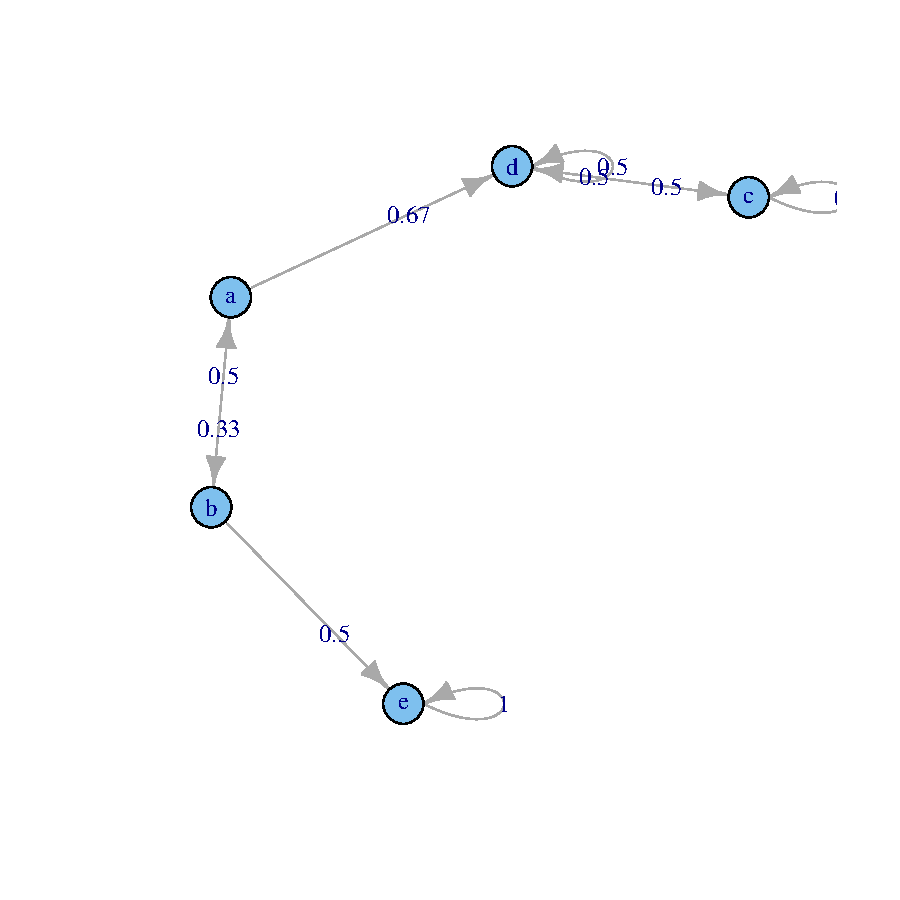
\includegraphics{an_introduction_to_markovchain_package-mathematica9McFig}
\caption{Mathematica 9 example. Markov chain plot.}
\label{fig:mcMathematics}
\end{center}
\end{figure}

\begin{Schunk}
\begin{Soutput}
Mathematica MC  Markov chain that is composed by: 
Closed classes: 
c d 
e 
Transient classes: 
a b 
The Markov chain is not irreducible 
The absorbing states are: e
\end{Soutput}
\end{Schunk}



\cite{renaldoMatlab} provides code to compute first passage time (within $1,2,\ldots, n$ steps) given the initial state to be $i$. The \proglang{MATLAB} listings translated into \proglang{R} on which the \code{firstPassage} function is based are

\begin{Schunk}
\begin{Sinput}
R> .firstpassageKernel <- function(P, i, n){
+    G <- P
+    H <- P[i,]
+    E <- 1 - diag(size(P)[2])
+    for (m in 2:n) {
+      G <- P %*% (G * E)
+      H <- rbind(H, G[i,])
+    }
+    return(H)
+  }
\end{Sinput}
\end{Schunk}

We conclude that the probability for the first rainy day to be the third one, given that the current state is sunny, is given by

\begin{Schunk}
\begin{Sinput}
R> firstPassagePdF <- firstPassage(object = mcWeather, state = "sunny", 
+                                  n = 10)
R> firstPassagePdF[3, 3]
\end{Sinput}
\begin{Soutput}
[1] 0.121
\end{Soutput}
\end{Schunk}



\section{Statistical analysis}\label{sec:statistics}

Table~\ref{tab:funs4Stats} lists the functions and methods implemented within
the package which help to fit, simulate and predict DTMC.

\begin{table}[h]
  \centering
  \begin{tabular}{lll}
    \hline
  Function & Purpose \\
    \hline  \hline
  \code{markovchainFit} & Function to return fitted Markov chain for a given sequence.\\
  \code{predict} & Method to calculate predictions from \code{markovchain} or
   \\
    & \code{markovchainList} objects.\\
   \code{rmarkovchain} & Function to sample from \code{markovchain} or \code{markovchainList} objects.\\
    \hline
\end{tabular}
\caption{The \pkg{markovchain} statistical functions.}
\label{tab:funs4Stats}
\end{table}  

\subsection{Simulation}

Simulating a random sequence from an underlying DTMC is quite easy thanks to the
function \code{rmarkovchain}. The following code generates a year
of weather states according to \code{mcWeather} underlying stochastic
process.

\begin{Schunk}
\begin{Sinput}
R> weathersOfDays <- rmarkovchain(n = 365, object = mcWeather, t0 = "sunny")
R> weathersOfDays[1:30]
\end{Sinput}
\begin{Soutput}
 [1] "sunny"  "cloudy" "sunny"  "sunny"  "cloudy" "rain"   "cloudy"
 [8] "sunny"  "rain"   "sunny"  "sunny"  "cloudy" "rain"   "cloudy"
[15] "sunny"  "sunny"  "sunny"  "sunny"  "sunny"  "sunny"  "rain"  
[22] "cloudy" "rain"   "cloudy" "cloudy" "rain"   "cloudy" "rain"  
[29] "cloudy" "rain"  
\end{Soutput}
\end{Schunk}

Similarly, it is possible to simulate one or more sequences from a non-homogeneous Markov chain, 
as the following code (applied on CCHC example) exemplifies.

\begin{Schunk}
\begin{Sinput}
R> patientStates <- rmarkovchain(n = 5, object = mcCCRC, t0 = "H", 
+                                include.t0 = TRUE)
R> patientStates[1:10,]
\end{Sinput}
\begin{Soutput}
   iteration values
1          1      H
2          1      D
3          1      D
4          1      D
5          1      D
6          2      H
7          2      H
8          2      H
9          2      H
10         2      D
\end{Soutput}
\end{Schunk}

\subsection{Estimation}

A time homogeneous Markov chain can be fit from given data. Four methods have been implemented within current version of
\pkg{markovchain} package: maximum likelihood, maximum likelihood with Laplace
smoothing, Bootstrap approach, maximum a posteriori. 

Equation~\ref{eq:MLE} shows the maximum likelihood estimator (MLE) of the
$p_{ij}$ entry, where the $n_{ij}$ element consists in the number sequences $\left( X_{t}=s_{i}, X_{t+1}=s_{j}\right)$
found in the sample, that is

\begin{equation}
{\hat p^{MLE}}_{ij} = \frac{{{n_{ij}}}}{{\sum\limits_{u = 1}^k {{n_{iu}}} }}.
\label{eq:MLE}
\end{equation}

Equation~\ref{eq:SE} shows the \code{standardError} of the MLE.

\begin{equation}
SE_{ij} = \frac{ {\hat p^{MLE}}_{ij} }{\sqrt{n_{ij}}}
\label{eq:SE}
\end{equation}

\begin{Schunk}
\begin{Sinput}
R> weatherFittedMLE <- markovchainFit(data = weathersOfDays, method = "mle",
+                                   name = "Weather MLE")
R> weatherFittedMLE$estimate
\end{Sinput}
\begin{Soutput}
Weather MLE 
 A  3 - dimensional discrete Markov Chain with following states 
 cloudy rain sunny 
 The transition matrix   (by rows)  is defined as follows 
          cloudy      rain     sunny
cloudy 0.3652174 0.3478261 0.2869565
rain   0.5517241 0.2988506 0.1494253
sunny  0.1604938 0.1296296 0.7098765
\end{Soutput}
\begin{Sinput}
R> weatherFittedMLE$standardError
\end{Sinput}
\begin{Soutput}
           cloudy       rain      sunny
cloudy 0.05635427 0.05499613 0.04995272
rain   0.07963452 0.05860942 0.04144312
sunny  0.03147543 0.02828750 0.06619633
\end{Soutput}
\end{Schunk}

The Laplace smoothing approach is a variation of the MLE, where the $n_{ij}$
is substituted by $n_{ij}+\alpha$ (see Equation~\ref{eq:LAPLACE}), being
$\alpha$ an arbitrary positive stabilizing parameter.

\begin{equation}
{\hat p^{LS}}_{ij} = \frac{{{n_{ij}} + \alpha }}{{\sum\limits_{u = 1}^k {\left( {{n_{iu}} + \alpha } \right)} }}
\label{eq:LAPLACE}
\end{equation}



\begin{Schunk}
\begin{Sinput}
R> weatherFittedLAPLACE <- markovchainFit(data = weathersOfDays, 
+                                      method = "laplace", laplacian = 0.01,
+                                      name = "Weather LAPLACE")
R> weatherFittedLAPLACE$estimate
\end{Sinput}
\begin{Soutput}
Weather LAPLACE 
 A  3 - dimensional discrete Markov Chain with following states 
 cloudy rain sunny 
 The transition matrix   (by rows)  is defined as follows 
          cloudy      rain     sunny
cloudy 0.3652091 0.3478223 0.2869686
rain   0.5516489 0.2988625 0.1494887
sunny  0.1605258 0.1296673 0.7098068
\end{Soutput}
\end{Schunk}


Both MLE and Laplace approach are based on the \code{createSequenceMatrix}
functions that converts a data (character) sequence into a contingency table,
showing the $\left( X_{t}=i, X_{t+1}=j\right)$ distribution within the sample,
as code below shows. 

\begin{Schunk}
\begin{Sinput}
R> createSequenceMatrix(stringchar = weathersOfDays)
\end{Sinput}
\begin{Soutput}
       cloudy rain sunny
cloudy     42   40    33
rain       48   26    13
sunny      26   21   115
\end{Soutput}
\end{Schunk}


An issue occurs when the sample contains only one realization of a state (say $X_{\beta}$) which is located at the end of the data sequence, since it yields to a row of zero (no sample to estimate the conditional
distribution of the transition). In this case the estimated transition matrix is
corrected assuming $p_{\beta,j}=1/k$, being $k$ the possible states.

A bootstrap estimation approach has been developed within the package in order
to provide an indication of the variability of ${\hat p}_{ij}$ estimates. The
bootstrap approach implemented within the \pkg{markovchain} package follows
these steps:

\begin{enumerate}
  \item bootstrap the data sequences following the conditional
  distributions of states estimated from the original one. The default bootstrap
  samples is 10, as specified in \code{nboot} parameter of \code{markovchainFit}
  function.
  \item apply MLE estimation on bootstrapped data sequences that are saved in
\\  \code{bootStrapSamples} slot of the returned list.
  \item the ${p^{BOOTSTRAP}}_{ij}$ is the average of all ${p^{MLE}}_{ij}$ across
  the \code{bootStrapSamples} list, normalized by row. A \code{standardError}
 of $\hat{{p^{MLE}}_{ij}}$ estimate is provided as well.
\end{enumerate}


\begin{Schunk}
\begin{Sinput}
R> weatherFittedBOOT <- markovchainFit(data = weathersOfDays, 
+                                      method = "bootstrap", nboot = 100)
R> weatherFittedBOOT$estimate
\end{Sinput}
\begin{Soutput}
BootStrap Estimate 
 A  3 - dimensional discrete Markov Chain with following states 
 cloudy rain sunny 
 The transition matrix   (by rows)  is defined as follows 
          cloudy      rain     sunny
cloudy 0.3679941 0.3499262 0.2820796
rain   0.5469893 0.3000676 0.1529431
sunny  0.1585844 0.1316045 0.7098111
\end{Soutput}
\begin{Sinput}
R> weatherFittedBOOT$standardError
\end{Sinput}
\begin{Soutput}
            cloudy        rain       sunny
cloudy 0.004395227 0.004305609 0.003707920
rain   0.005762406 0.005241380 0.003929288
sunny  0.002853011 0.002808520 0.003823990
\end{Soutput}
\end{Schunk}

The bootstrapping process can be done in \code{parallel}.

\begin{Schunk}
\begin{Sinput}
R> weatherFittedBOOTParallel <- markovchainFit(data = weathersOfDays, 
+                                      method = "bootstrap", nboot = 10, 
+                                      parallel = TRUE)
R> weatherFittedBOOTParallel$estimate
R> weatherFittedBOOTParallel$standardError
\end{Sinput}
\end{Schunk}

The parallel bootstrapping uses all the available cores on a machine by default.
However, it is also possible to tune the number of threads used. 
Note that this should be done in R before calling the \code{markovchainFit} function.
For example, the following code will set the number of threads to 4.

\begin{Schunk}
\begin{Sinput}
R> RcppParallel::setNumThreads(4)
\end{Sinput}
\end{Schunk}

For more details, please refer to \pkg{RcppParallel} (http://rcppcore.github.io/RcppParallel/).


For all the fitting methods, the \code{logLikelihood} denoted in Equation~\ref{eq:LLH} is provided. 

\begin{equation}
LLH = \sum_{i,j} n_{ij} * log (p_{ij})
\label{eq:LLH}
\end{equation}
where $n_{ij}$ is the entry of the frequency matrix and $p_{ij}$ is the entry of the transition probability matrix.

\begin{Schunk}
\begin{Sinput}
R> weatherFittedMLE$logLikelihood
\end{Sinput}
\begin{Soutput}
[1] -340.2846
\end{Soutput}
\begin{Sinput}
R> weatherFittedBOOT$logLikelihood
\end{Sinput}
\begin{Soutput}
[1] -340.3011
\end{Soutput}
\end{Schunk}

Confidence matrices of estimated parameters (parametric for MLE, non - parametric for BootStrap) are available as well.

\begin{Schunk}
\begin{Sinput}
R> weatherFittedMLE$confidenceInterval
\end{Sinput}
\begin{Soutput}
$confidenceLevel
[1] 0.95

$lowerEndpointMatrix
          cloudy       rain      sunny
cloudy 0.2725229 0.25736550 0.20479161
rain   0.4207370 0.20244666 0.08125742
sunny  0.1087214 0.08310083 0.60099327

$upperEndpointMatrix
          cloudy      rain     sunny
cloudy 0.4579119 0.4382867 0.3691214
rain   0.6827113 0.3952545 0.2175932
sunny  0.2122663 0.1761584 0.8187598
\end{Soutput}
\begin{Sinput}
R> weatherFittedBOOT$confidenceInterval
\end{Sinput}
\begin{Soutput}
$confidenceLevel
[1] 0.95

$lowerEndpointMatrix
          cloudy      rain     sunny
cloudy 0.3607646 0.3428441 0.2759807
rain   0.5375110 0.2914463 0.1464800
sunny  0.1538916 0.1269849 0.7035212

$upperEndpointMatrix
          cloudy      rain     sunny
cloudy 0.3752236 0.3570083 0.2881786
rain   0.5564676 0.3086889 0.1594062
sunny  0.1632772 0.1362241 0.7161010
\end{Soutput}
\end{Schunk}


The functions for fitting DTMC have mostly been rewritten in \proglang{C++} using \pkg{Rcpp} \cite{RcppR} since version 0.2.\\

Is is also possible to fit a DTMC or a \code{markovchainList} object 
from \code{matrix} or \code{data.frame} objects as shown in following code.

\begin{Schunk}
\begin{Sinput}
R> data(holson)
R> singleMc<-markovchainFit(data=holson[,2:12],name="holson")
R> mcListFit<-markovchainListFit(data=holson[,2:12],name="holson")
R> mcListFit$estimate[[1]]
\end{Sinput}
\begin{Soutput}
time1 
 A  3 - dimensional discrete Markov Chain with following states 
 1 2 3 
 The transition matrix   (by rows)  is defined as follows 
           1          2         3
1 0.94609164 0.05390836 0.0000000
2 0.26356589 0.62790698 0.1085271
3 0.02325581 0.18604651 0.7906977
\end{Soutput}
\end{Schunk}




The maximum a posteriori method (MAP) has been implemented using Bayesian inference \citep{sch}. For details on usage, refer to the stand-alone vignette for MAP \citep{MAPmcR}.

\subsection{Prediction}


The $n$-step forward predictions can be obtained using the \code{predict} methods
explicitly written for \code{markovchain} and \code{markovchainList} objects. 
The prediction is the mode of the conditional distribution of $X_{t+1}$ given
$X_{t}=s_{j}$, being $s_{j}$ the last realization of the DTMC (homogeneous
or non-homogeneous).

\subsubsection{Predicting from a markovchain object}

The 3-days forward predictions from \code{markovchain} object can be generated as follows, assuming that the last two days were respectively "cloudy" and "sunny".

\begin{Schunk}
\begin{Sinput}
R> predict(object = weatherFittedMLE$estimate, newdata = c("cloudy", "sunny"),
+          n.ahead = 3)
\end{Sinput}
\begin{Soutput}
[1] "sunny" "sunny" "sunny"
\end{Soutput}
\end{Schunk}

\subsubsection{Predicting from a markovchainList object}

Given an initial two year Healty status, the 5-year ahead prediction of any
CCRC guest is

\begin{Schunk}
\begin{Sinput}
R> predict(mcCCRC, newdata = c("H", "H"), n.ahead = 5)
\end{Sinput}
\begin{Soutput}
[1] "H" "D" "D"
\end{Soutput}
\end{Schunk}

The prediction has stopped at time sequence since the underlying
non-homogeneous Markov chain has a length of four. In order to continue five
years ahead, the \code{continue=TRUE} parameter setting makes the \code{predict}
method keeping to use the last \code{markovchain} in the sequence list.


\begin{Schunk}
\begin{Sinput}
R> predict(mcCCRC, newdata = c("H", "H"), n.ahead = 5, continue = TRUE)
\end{Sinput}
\begin{Soutput}
[1] "H" "D" "D" "D" "D"
\end{Soutput}
\end{Schunk}

\section{Applications}\label{sec:applications}

This section shows applications of DTMC in various
fields.

\subsection{Weather forecasting}\label{app:weather}

Markov chains provide a simple model to predict the next day's weather given the
current meteorological condition.
The first application herewith shown is the "Land of Oz example" from \cite{landOfOz}, the second is the "Alofi Island Rainfall" from \cite{averyHenderson}.

\subsubsection{Land of Oz}\label{sec:wfLandOfOz}

The Land of Oz is 
acknowledged not to have ideal weather conditions at all: 
the weather is snowy or rainy very often and, once more, there are never two
nice days in a row. Consider three weather states: rainy, nice and snowy. Let the transition matrix be as in the following:

\begin{Schunk}
\begin{Sinput}
R> mcWP <- new("markovchain", states = c("rainy", "nice", "snowy"),
+           transitionMatrix = matrix(c(0.5, 0.25, 0.25,
+                                     0.5, 0, 0.5,
+                                     0.25,0.25,0.5), byrow = T, nrow = 3))
\end{Sinput}
\end{Schunk}

Given that today it is a nice day, the corresponding stochastic row vector is
$w_{0}=(0\:,1\:,0)$ and the forecast after 1, 2 and 3 days are given by

\begin{Schunk}
\begin{Sinput}
R> W0 <- t(as.matrix(c(0, 1, 0)))
R> W1 <- W0 * mcWP; W1
\end{Sinput}
\begin{Soutput}
     rainy nice snowy
[1,]   0.5    0   0.5
\end{Soutput}
\begin{Sinput}
R> W2 <- W0 * (mcWP ^ 2); W2
\end{Sinput}
\begin{Soutput}
     rainy nice snowy
[1,] 0.375 0.25 0.375
\end{Soutput}
\begin{Sinput}
R> W3 <- W0 * (mcWP ^ 3); W3
\end{Sinput}
\begin{Soutput}
       rainy   nice   snowy
[1,] 0.40625 0.1875 0.40625
\end{Soutput}
\end{Schunk}

As can be seen from $w_{1}$, if in the Land of Oz today is a nice day, tomorrow it will rain or snow with probability 1. One week later, the prediction can be computed as

\begin{Schunk}
\begin{Sinput}
R> W7 <- W0 * (mcWP ^ 7)
R> W7
\end{Sinput}
\begin{Soutput}
         rainy      nice     snowy
[1,] 0.4000244 0.1999512 0.4000244
\end{Soutput}
\end{Schunk}

The steady state of the chain can be computed by means of the \code{steadyStates} method.

\begin{Schunk}
\begin{Sinput}
R> q <- steadyStates(mcWP)
R> q
\end{Sinput}
\begin{Soutput}
     rainy nice snowy
[1,]   0.4  0.2   0.4
\end{Soutput}
\end{Schunk}

Note that, from the seventh day on, the predicted probabilities are substantially equal to the steady state of the chain and they don't depend from the starting point, as the following code shows.


\begin{Schunk}
\begin{Sinput}
R> R0 <- t(as.matrix(c(1, 0, 0)))
R> R7 <- R0 * (mcWP ^ 7); R7
\end{Sinput}
\begin{Soutput}
         rainy      nice     snowy
[1,] 0.4000244 0.2000122 0.3999634
\end{Soutput}
\begin{Sinput}
R> S0 <- t(as.matrix(c(0, 0, 1)))
R> S7 <- S0 * (mcWP ^ 7); S7
\end{Sinput}
\begin{Soutput}
         rainy      nice     snowy
[1,] 0.3999634 0.2000122 0.4000244
\end{Soutput}
\end{Schunk}

\subsubsection{Alofi Island Rainfall}\label{sec:wfAlofi}

Alofi Island daily rainfall
data were recorded from January 1st, 1987 until December 31st, 1989 and
classified into three states: "0" (no rain), "1-5" (from non zero until 5 mm) and "6+" (more than 5mm). The corresponding dataset is provided within the
\pkg{markovchain} package.

\begin{Schunk}
\begin{Sinput}
R> data("rain", package = "markovchain")
R> table(rain$rain)
\end{Sinput}
\begin{Soutput}
  0 1-5  6+ 
548 295 253 
\end{Soutput}
\end{Schunk}

The underlying transition matrix is estimated as follows.

\begin{Schunk}
\begin{Sinput}
R> mcAlofi <- markovchainFit(data = rain$rain, name = "Alofi MC")$estimate
R> mcAlofi
\end{Sinput}
\begin{Soutput}
Alofi MC 
 A  3 - dimensional discrete Markov Chain with following states 
 0 1-5 6+ 
 The transition matrix   (by rows)  is defined as follows 
            0       1-5        6+
0   0.6605839 0.2299270 0.1094891
1-5 0.4625850 0.3061224 0.2312925
6+  0.1976285 0.3122530 0.4901186
\end{Soutput}
\end{Schunk}

The long term daily rainfall distribution is obtained by means of the \code{steadyStates} method.

\begin{Schunk}
\begin{Sinput}
R> steadyStates(mcAlofi)
\end{Sinput}
\begin{Soutput}
             0       1-5        6+
[1,] 0.5008871 0.2693656 0.2297473
\end{Soutput}
\end{Schunk}


\subsection{Finance and Economics}\label{app:fin}

Other relevant applications of DTMC can be found in Finance and Economics.

\subsubsection{Finance}\label{fin:fin}

Credit ratings transitions have been successfully modelled with discrete time Markov chains. Some rating agencies publish transition matrices that show the empirical transition probabilities across credit ratings. The example that follows 
comes from \pkg{CreditMetrics} \proglang{R} package \citep{CreditMetricsR},
carrying Standard \& Poor's published data.

\begin{Schunk}
\begin{Sinput}
R> rc <- c("AAA", "AA", "A", "BBB", "BB", "B", "CCC", "D")
R> creditMatrix <- matrix(c(90.81, 8.33, 0.68, 0.06, 0.08, 0.02, 0.01, 0.01,
+  0.70, 90.65, 7.79, 0.64, 0.06, 0.13, 0.02, 0.01,
+  0.09, 2.27, 91.05, 5.52, 0.74, 0.26, 0.01, 0.06,
+  0.02, 0.33, 5.95, 85.93, 5.30, 1.17, 1.12, 0.18,
+  0.03, 0.14, 0.67, 7.73, 80.53, 8.84, 1.00, 1.06,
+  0.01, 0.11, 0.24, 0.43, 6.48, 83.46, 4.07, 5.20,
+  0.21, 0, 0.22, 1.30, 2.38, 11.24, 64.86, 19.79,
+  0, 0, 0, 0, 0, 0, 0, 100
+  )/100, 8, 8, dimnames = list(rc, rc), byrow = TRUE)
\end{Sinput}
\end{Schunk}

It is easy to convert such matrices into \code{markovchain} objects and to perform some analyses

\begin{Schunk}
\begin{Sinput}
R> creditMc <- new("markovchain", transitionMatrix = creditMatrix, 
+                  name = "S&P Matrix")
R> absorbingStates(creditMc)
\end{Sinput}
\begin{Soutput}
[1] "D"
\end{Soutput}
\end{Schunk}

\subsubsection{Economics}\label{fin:ec}

For a recent application of \pkg{markovchain} in Economic, see \cite{manchesterR}. 

A dynamic system generates two kinds of economic effects \citep{bardPpt}:
\begin{enumerate}
\item those incurred when the system is in a specified state, and
\item those incurred when the system makes a transition from one state to another.
\end{enumerate}

Let the monetary amount of being in a particular state be represented as a m-dimensional column vector $c^{\rm{S}}$, while let the monetary amount of a transition be embodied in a $C^{R}$ matrix in which each component specifies the monetary amount of going from state i to state j in a single step. Henceforth, Equation~\ref{eq:cost} represents the monetary of being in state $i$.

\begin{equation}
{c_i} = c_i^{\rm{S}} + \sum\limits_{j = 1}^m {C_{ij}^{\rm{R}}} {p_{ij}}.
\label{eq:cost}
\end{equation}

Let $\bar c = \left[ c_i \right]$ and let $e_i$ be the vector valued 1 in the initial state and 0 in all other, then, if $f_n$ is the random variable representing the economic return associated with the stochastic process at time $n$, Equation~\ref{eq:return} holds:

\begin{equation}
E\left[ {{f_n}\left( {{X_n}} \right)|{X_0} = i} \right] = {e_i}{P^n}\bar c.
\label{eq:return}
\end{equation}

The following example assumes that a telephone company models the transition probabilities between customer/non-customer status by matrix $P$ and the cost associated to states by matrix $M$.

\begin{Schunk}
\begin{Sinput}
R> statesNames <- c("customer", "non customer")
R> P <- zeros(2); P[1, 1] <- .9; P[1, 2] <- .1; P[2, 2] <- .95; P[2, 1] <- .05;
R> rownames(P) <- statesNames; colnames(P) <- statesNames
R> mcP <- new("markovchain", transitionMatrix = P, name = "Telephone company")
R> M <- zeros(2); M[1, 1] <- -20; M[1, 2] <- -30; M[2, 1] <- -40; M[2, 2] <- 0
\end{Sinput}
\end{Schunk}

If the average revenue for existing customer is +100, the cost per state is computed as follows.

\begin{Schunk}
\begin{Sinput}
R> c1 <- 100 + conditionalDistribution(mcP, state = "customer") %*% M[1,]
R> c2 <- 0 + conditionalDistribution(mcP, state = "non customer") %*% M[2,]
\end{Sinput}
\end{Schunk}

For an existing customer, the expected gain (loss) at the fifth year is given by the following code.

\begin{Schunk}
\begin{Sinput}
R> as.numeric((c(1, 0)* mcP ^ 5) %*% (as.vector(c(c1, c2))))
\end{Sinput}
\begin{Soutput}
[1] 48.96009
\end{Soutput}
\end{Schunk}
\subsection{Actuarial science}\label{app:act}

Markov chains are widely applied in the field of actuarial science. Two
classical applications are policyholders' distribution across Bonus Malus
classes in Motor Third Party Liability (MTPL) insurance (Section~\ref{sec:bm}) and health insurance pricing and reserving 
(Section~\ref{sec:hi}).


\subsubsection{MPTL Bonus Malus}\label{sec:bm}

Bonus Malus (BM) contracts grant the policyholder a discount (enworsen) as a
function of the number of claims in the experience period. The discount (enworsen) is applied on a premium that 
already allows for known (a priori) policyholder characteristics \citep{denuit2007actuarial}
and it usually depends on vehicle, territory, the demographic profile of the policyholder, and policy coverages deep (deductible and policy limits).\\
Since the proposed BM level depends on the claim on the previous period, it can
be modelled by a discrete Markov chain. A very simplified example follows.
Assume a BM scale from 1 to 5, where 4 is the starting level. The evolution rules are shown in Equation~\ref{eq:BM}:

\begin{equation}
bm_{t + 1} = \max \left( {1,bm_{t} - 1} \right)*\left( {\tilde N = 0} \right) + \min \left( {5,bm_{t} + 2*\tilde N} \right)*\left( {\tilde N \ge 1} \right).
\label{eq:BM}
\end{equation}

Tthe number of claim $\tilde N$  is a random variable that is assumed
to be Poisson distributed.

\begin{Schunk}
\begin{Sinput}
R> getBonusMalusMarkovChain <- function(lambda)
+  {
+  	bmMatr <- zeros(5)
+  	bmMatr[1, 1] <- dpois(x = 0, lambda)
+  	bmMatr[1, 3] <- dpois(x = 1, lambda)
+  	bmMatr[1, 5] <- 1 - ppois(q = 1, lambda)
+  	
+  	bmMatr[2, 1] <- dpois(x = 0, lambda)
+  	bmMatr[2, 4] <- dpois(x = 1, lambda)
+  	bmMatr[2, 5] <- 1 - ppois(q = 1, lambda)
+  	
+  	bmMatr[3, 2] <- dpois(x = 0, lambda)
+  	bmMatr[3, 5] <- 1 - dpois(x=0, lambda)
+   
+  	bmMatr[4, 3] <- dpois(x = 0, lambda)
+  	bmMatr[4, 5] <- 1 - dpois(x = 0, lambda)
+    
+  	bmMatr[5, 4] <- dpois(x = 0, lambda)
+  	bmMatr[5, 5] <- 1 - dpois(x = 0, lambda)
+  	stateNames <- as.character(1:5)
+  	out <- new("markovchain", transitionMatrix = bmMatr, 
+               states = stateNames, name = "BM Matrix")
+  	return(out)
+  }
R> 
\end{Sinput}
\end{Schunk}

Assuming that the a-priori claim frequency per car-year is 0.05 in the class (being the class the group of policyholders that share the same common characteristics), the underlying BM transition matrix and its underlying steady state are as follows.

\begin{Schunk}
\begin{Sinput}
R> bmMc <- getBonusMalusMarkovChain(0.05)
R> as.numeric(steadyStates(bmMc))
\end{Sinput}
\begin{Soutput}
[1] 0.895836079 0.045930498 0.048285405 0.005969247 0.003978772
\end{Soutput}
\end{Schunk}

If the underlying BM coefficients of the class are 0.5, 0.7, 0.9, 1.0, 1.25, this
means that the average BM coefficient applied on the long run to the class is given by

\begin{Schunk}
\begin{Sinput}
R> sum(as.numeric(steadyStates(bmMc)) * c(0.5, 0.7, 0.9, 1, 1.25))
\end{Sinput}
\begin{Soutput}
[1] 0.534469
\end{Soutput}
\end{Schunk}

This means that the average premium paid by policyholders in the portfolio
almost halves in the long run.

\subsubsection{Health insurance example}\label{sec:hi}
Actuaries quantify the risk inherent in insurance contracts evaluating the premium of insurance contract to be sold (therefore covering future risk) and evaluating the actuarial reserves of existing portfolios (the liabilities in terms of benefits or claims payments due to policyholder arising from previously sold contracts).
Key quantities of actuarial interest are: the expected present value of future benefits, $PVFB$, the (periodic) benefit premium, $P$, and the present value of future premium $PVFP$. A level benefit premium could be set equating at the beginning of the contract $PVFB=PVFP$. After the beginning of the contract the benefit reserve is the difference between $PVFB$ and $PVFP$.
The example comes from \cite{deshmukh2012multiple}. The interest rate is 5\%, 
benefits are payable upon death (1000) and disability (500). Premiums are 
payable at the beginning of period only if the policyholder is active. The contract term is three years.

\begin{Schunk}
\begin{Sinput}
R> mcHI <- new("markovchain", states = c("active", "disable", "withdrawn", 
+                                        "death"),
+           transitionMatrix = matrix(c(0.5, .25, .15, .1,
+                                     0.4, 0.4, 0.0, 0.2,
+                                     0, 0, 1, 0,
+                                     0, 0, 0, 1), byrow = TRUE, nrow = 4))
R> benefitVector <- as.matrix(c(0, 0, 500, 1000))
\end{Sinput}
\end{Schunk}

The policyholders is active at $T_0$. Therefore the expected states at $T_1, \ldots T_3$ are calculated in the following.

\begin{Schunk}
\begin{Sinput}
R> T0 <- t(as.matrix(c(1, 0, 0, 0)))
R> T1 <- T0 * mcHI
R> T2 <- T1 * mcHI
R> T3 <- T2 * mcHI
\end{Sinput}
\end{Schunk}

The present value of future benefit at T0 is given by

\begin{Schunk}
\begin{Sinput}
R> PVFB <- T0 %*% benefitVector * 1.05 ^ -0 + 
+    T1 %*% benefitVector * 1.05 ^ -1+
+    T2 %*% benefitVector * 1.05 ^ -2 + T3 %*% benefitVector * 1.05 ^ -3
\end{Sinput}
\end{Schunk}

The yearly premium payable whether the insured is alive is as follows. 

\begin{Schunk}
\begin{Sinput}
R> P <- PVFB / (T0[1] * 1.05 ^- 0 + T1[1] * 1.05 ^ -1 + T2[1] * 1.05 ^ -2)
\end{Sinput}
\end{Schunk}

The reserve at the beginning of the second year, in the case of the insured being alive, is as follows.

\begin{Schunk}
\begin{Sinput}
R> PVFB <- T2 %*% benefitVector * 1.05 ^ -1 + T3 %*% benefitVector * 1.05 ^ -2
R> PVFP <- P*(T1[1] * 1.05 ^ -0 + T2[1] * 1.05 ^ -1)
R> V <- PVFB - PVFP
R> V
\end{Sinput}
\begin{Soutput}
         [,1]
[1,] 300.2528
\end{Soutput}
\end{Schunk}

\subsection{Sociology}\label{app:sociology}

Markov chains have been actively used to model progressions and regressions between social classes. The first study was performed by \cite{glassHall}, while a more recent application can be found in \cite{blandenEtAlii}. The table that follows shows the income quartile of the father when the son was 16 (in 1984) and the income quartile of the son when aged 30 (in 2000) for the 1970 cohort.

\begin{Schunk}
\begin{Sinput}
R> data("blanden")
R> mobilityMc <- as(blanden, "markovchain")
R> mobilityMc
\end{Sinput}
\begin{Soutput}
Unnamed Markov chain 
 A  4 - dimensional discrete Markov Chain with following states 
 Bottom 2nd 3rd Top 
 The transition matrix   (by rows)  is defined as follows 
             2nd       3rd    Bottom       Top
Bottom 0.2900000 0.2200000 0.3800000 0.1100000
2nd    0.2772277 0.2574257 0.2475248 0.2178218
3rd    0.2626263 0.2828283 0.2121212 0.2424242
Top    0.1700000 0.2500000 0.1600000 0.4200000
\end{Soutput}
\end{Schunk}

The underlying transition graph is plotted in Figure~\ref{fig:mobility}.

\begin{figure}
\begin{center}
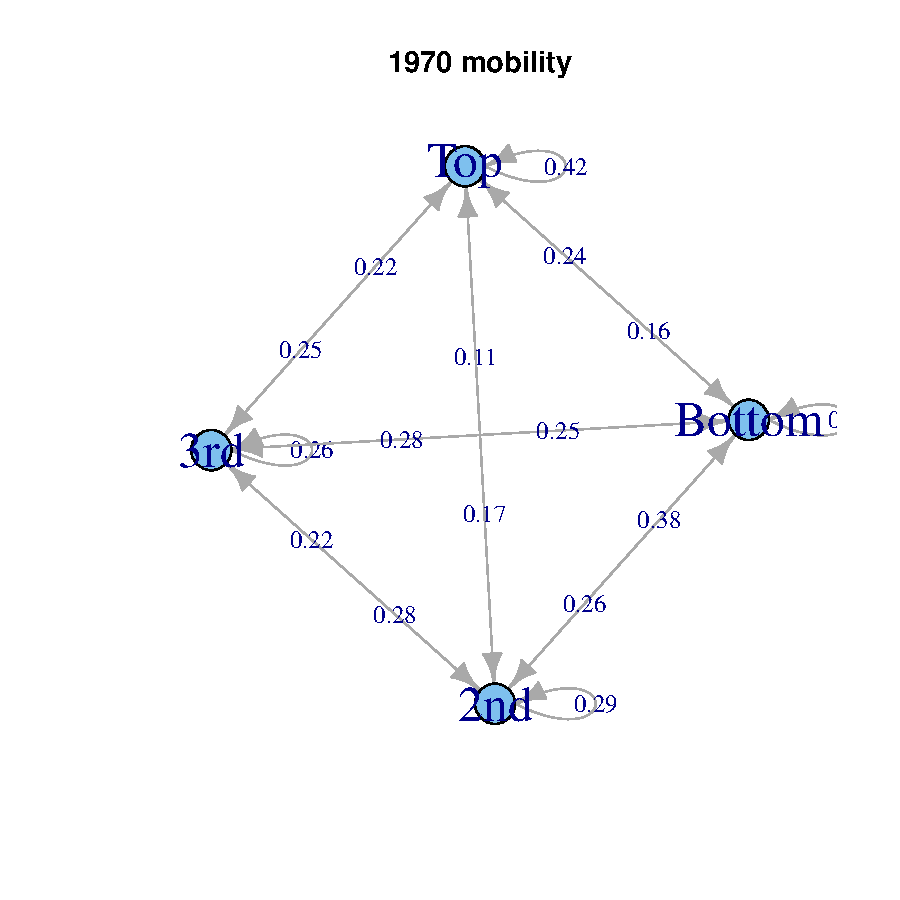
\includegraphics{an_introduction_to_markovchain_package-blandenEtAlii2}
\caption{1970 UK cohort mobility data.}
\label{fig:mobility}
\end{center}
\end{figure}

The steady state distribution is computed as follows. Since transition across
quartiles are shown, the probability function is evenly 0.25.

\begin{Schunk}
\begin{Sinput}
R> round(steadyStates(mobilityMc), 2)
\end{Sinput}
\begin{Soutput}
     Bottom  2nd  3rd  Top
[1,]   0.25 0.25 0.25 0.25
\end{Soutput}
\end{Schunk}

\subsection{Genetics and Medicine}\label{sec:gen}

This section contains two examples: the first shows the use of Markov chain
models in genetics, the second shows an application
of Markov chains in modelling diseases' dynamics.


\subsubsection{Genetics}\label{sec:genetics}

\cite{averyHenderson} discusses the use of Markov chains in model Preprogucacon
gene protein bases sequence. The \code{preproglucacon} dataset in \pkg{markovchain}
contains the dataset shown in the package.

\begin{Schunk}
\begin{Sinput}
R> data("preproglucacon", package = "markovchain")
\end{Sinput}
\end{Schunk}

It is possible to model the transition probabilities between bases as shown in the following code.

\begin{Schunk}
\begin{Sinput}
R> mcProtein <- markovchainFit(preproglucacon$preproglucacon, 
+                            name = "Preproglucacon MC")$estimate
R> mcProtein
\end{Sinput}
\begin{Soutput}
Preproglucacon MC 
 A  4 - dimensional discrete Markov Chain with following states 
 A C G T 
 The transition matrix   (by rows)  is defined as follows 
          A         C          G         T
A 0.3585271 0.1434109 0.16666667 0.3313953
C 0.3840304 0.1558935 0.02281369 0.4372624
G 0.3053097 0.1991150 0.15044248 0.3451327
T 0.2844523 0.1819788 0.17667845 0.3568905
\end{Soutput}
\end{Schunk}

\subsubsection{Medicine}\label{sec:medicine}

Discrete-time Markov chains are also employed to study the progression of chronic diseases.
The following example is taken from \cite{craigSendi}. Starting from six month follow-up data, the maximum likelihood estimation
of the monthly transition matrix is obtained. This transition matrix aims to describe the monthly progression of CD4-cell counts of HIV infected subjects.

\begin{Schunk}
\begin{Sinput}
R> craigSendiMatr <- matrix(c(682, 33, 25,
+                154, 64, 47,
+                19, 19, 43), byrow = T, nrow = 3)
R> hivStates <- c("0-49", "50-74", "75-UP")
R> rownames(craigSendiMatr) <- hivStates
R> colnames(craigSendiMatr) <- hivStates
R> craigSendiTable <- as.table(craigSendiMatr)
R> mcM6 <- as(craigSendiTable, "markovchain")
R> mcM6@name <- "Zero-Six month CD4 cells transition"
R> mcM6
\end{Sinput}
\begin{Soutput}
Zero-Six month CD4 cells transition 
 A  3 - dimensional discrete Markov Chain with following states 
 0-49 50-74 75-UP 
 The transition matrix   (by rows)  is defined as follows 
           0-49      50-74      75-UP
0-49  0.9216216 0.04459459 0.03378378
50-74 0.5811321 0.24150943 0.17735849
75-UP 0.2345679 0.23456790 0.53086420
\end{Soutput}
\end{Schunk}

As shown in the paper, the second passage consists in the decomposition of
$M_{6}=V \cdot D \cdot V^{-1}$ in order to obtain $M_{1}$ as $M_{1}=V \cdot D^{1/6} \cdot V^{-1}$ .

\begin{Schunk}
\begin{Sinput}
R> eig <- eigen(mcM6@transitionMatrix)
R> D <- diag(eig$values)
\end{Sinput}
\end{Schunk}

\begin{Schunk}
\begin{Sinput}
R> V <- eig$vectors 
R> V %*% D %*% solve(V)
\end{Sinput}
\begin{Soutput}
          [,1]       [,2]       [,3]
[1,] 0.9216216 0.04459459 0.03378378
[2,] 0.5811321 0.24150943 0.17735849
[3,] 0.2345679 0.23456790 0.53086420
\end{Soutput}
\begin{Sinput}
R> d <- D ^ (1/6)
R> M <- V %*% d %*% solve(V)
R> mcM1 <- new("markovchain", transitionMatrix = M, states = hivStates)
\end{Sinput}
\end{Schunk}



\section{Discussion, issues and future plans}

The \pkg{markovchain} package has been designed in order to provide easily handling of DTMC and communication with alternative packages.

Some numerical issues have been found when working with matrix algebra using
\proglang{R} internal linear algebra kernel (the same calculations performed
with \proglang{MATLAB} gave a more accurate result).
Some temporary workarounds have been implemented. For example, the condition for row/column sums to be equal to
one is valid up to fifth decimal. Similarly, when extracting the eigenvectors
only the real part is taken.

Such limitations are expected to be overcome in future releases. Similarly,
future versions of the package are expected to improve the code in terms of numerical accuracy and rapidity.
An intitial rewriting of internal function in \proglang{C++} by means of \pkg{Rcpp} package \citep{RcppR} has been started.


\section*{Aknowledgments}\label{sec:aknowledgements}

The author wishes to thank Michael Cole, Tobi Gutman and Mildenberger Thoralf for their suggestions and bug checks. A very special thanks also to Tae Seung Kang (and to the other Google Summer of Code 2015 candidates) for having rewritten the fitting functions into \pkg{Rcpp}. A final thanks also to Dr. Simona C. Minotti and Dr. Mirko Signorelli for their support in drafting this version of the vignettes.   

\bibliography{markovchainBiblio}



\end{document}
